%\emph{(En esta subsección se deben describir y justificar los metodos de desarrollo y/o investigación que se aplicaran a lo largo del desarrollo del proyecto.)}

%\emph{(La longitud máxima de esta sección es de 1 página.)}

La metodología a utilizar será la metodología de desarrollo ágil Melé. \cite{7}

Los principios de esta metodología guían las actividades dentro de un proceso que incorpora las siguientes actividades del marco de trabajo: \emph{(requisitos, análisis, diseño, evolución y entrega)}. En cada actividad del marco de trabajo las tareas de trabajo suceden dentro del patrón de proceso llamado \emph{Sprint}. El trabajo realizado en un Sprint se adapta al problema y con frecuencia se modifica en tiempo real.

\begin{figure}[!hb]
	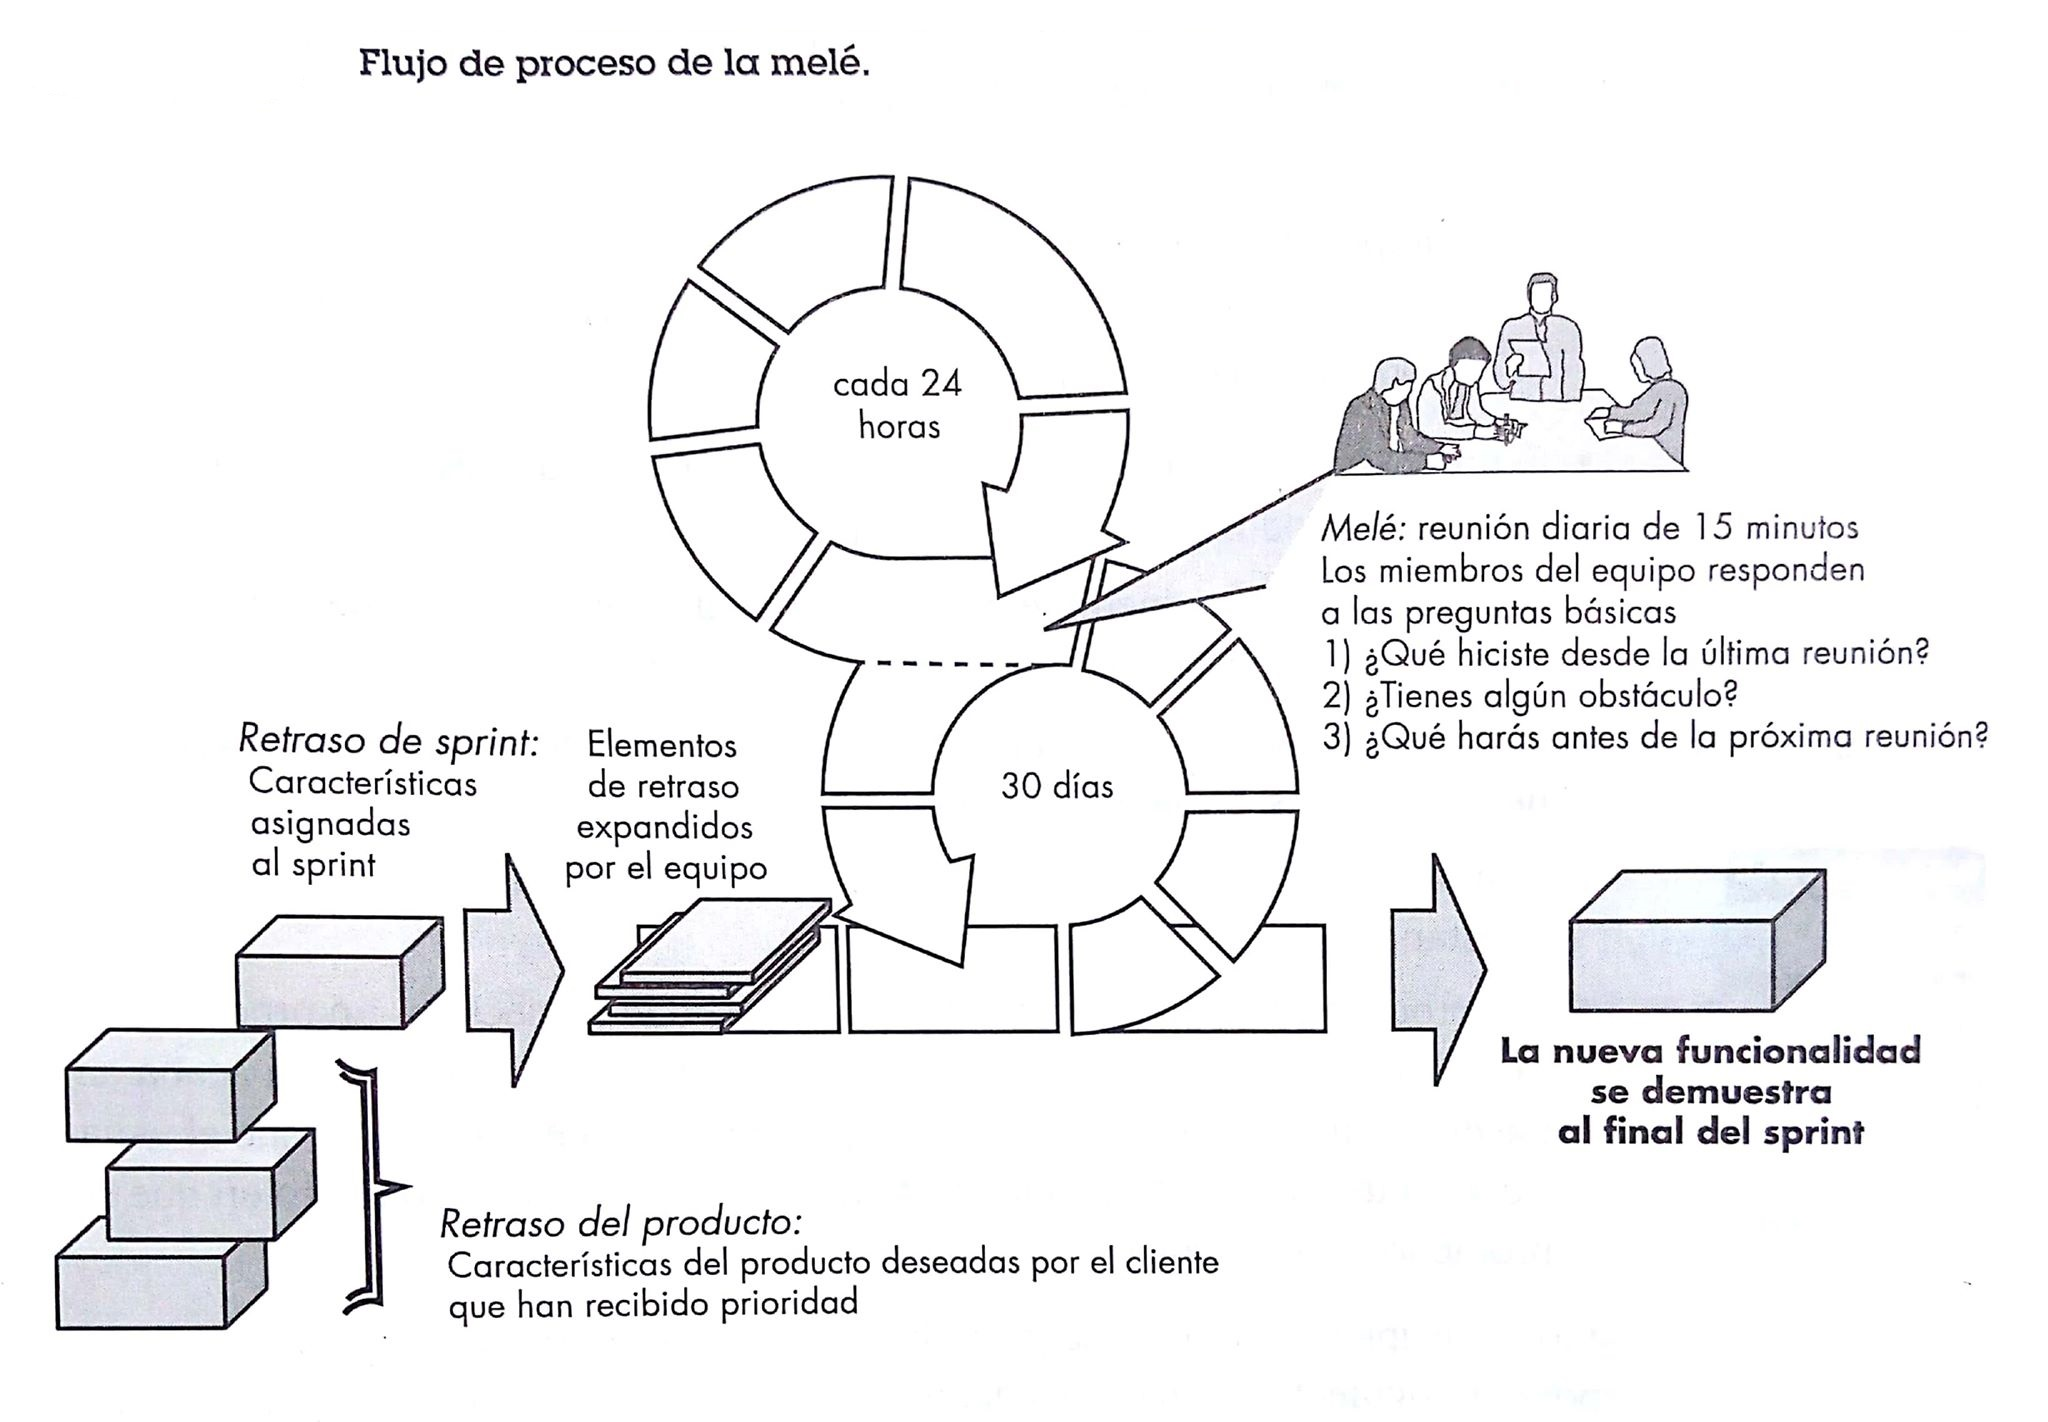
\includegraphics[width=\textwidth]{Imagenes/mele.jpg}
	\label{}
	\caption{Proceso de metodología Melé}
\end{figure}

Melé tiene un conjunto de \emph{"patrones de proceso de software"} los cuales define un conjunto de actividades de desarrollo:

\begin{itemize}
	\item 	\begin{description}
			    \item[Retrasos:] son una lista que considera la prioridad de los requisitos o características del proyecto que proporcionan valor comercial para el cliente. En cualquier momento se pueden agregar elementos a os retrasos. El gerente de producto evalúa los retrasos y actualiza las prioridades de acuerdo con lo requerido. 
			\end{description}

	\item 	\begin{description}
			    \item[Sprint:] consiste en unidades de trabajo que se requieren para satisfacer un requisito definido en los retrasos en un periodo predefinido (el lapso usual es de 30 días). En esta etapa, los elementos de los retrasos a los que se dirigen las unidades de trabajo del Sprint están congelados (es decir, durante le Sprint no se introducen cambios). Por lo tanto, el Sprint permite trabajar en un ambiente enfocado al corto plazo, pero estable.
			\end{description}

	\item 	\begin{description}
			    \item[Reuniones:] reuniones cortas (por lo general 15 minutos) y las realiza a diario el equipo de Melé. Existen 3 preguntas que plantean y responden todos los miembros del equipo:

			    \begin{itemize}
			    	\item ¿Qué hiciste desde la semana pasada?

			    	\item ¿Cuáles obstáculos encontraste? 

			    	\item ¿Qué esperas lograr para la siguiente reunión del equipo?
			    \end{itemize}

			 	Cada reunión ayuda a descubrir problemas potenciales tan pronto sea posible.
			\end{description}

	\item 	\begin{description}
			    \item[Demostración:] se entrega el incremento del software al cliente de forma que éste demuestre y evalúe la funcionalidad implementada. Es importante señalar que la demostración quizá no contenga toda la funcionalidad planteada, sino aquellas funciones susceptibles de entregarse dentro del periodo establecido.
			\end{description}
\end{itemize}



Los motivos por los cuales este método se implementará son:

\begin{itemize}
	\item Completa participación del cliente y prueba de funcionalidades para obtener retroalimentación.

	\item Se pueden obtener los cambios y adaptarse al proyecto en cada Sprint.

	\item Como la idea principal es realizar rendiciones y se han aclarado algunos requerimientos, más no son todos, es que se espera que el proyecto aumente en el proceso de desarrollo. Es por esta incertidumbre que se escoge la metodología Melé, ya que ayuda al cliente y al equipo de trabajo a definir los requisitos del proyecto.
\end{itemize}

%\begin{figure}
%  \centering
%    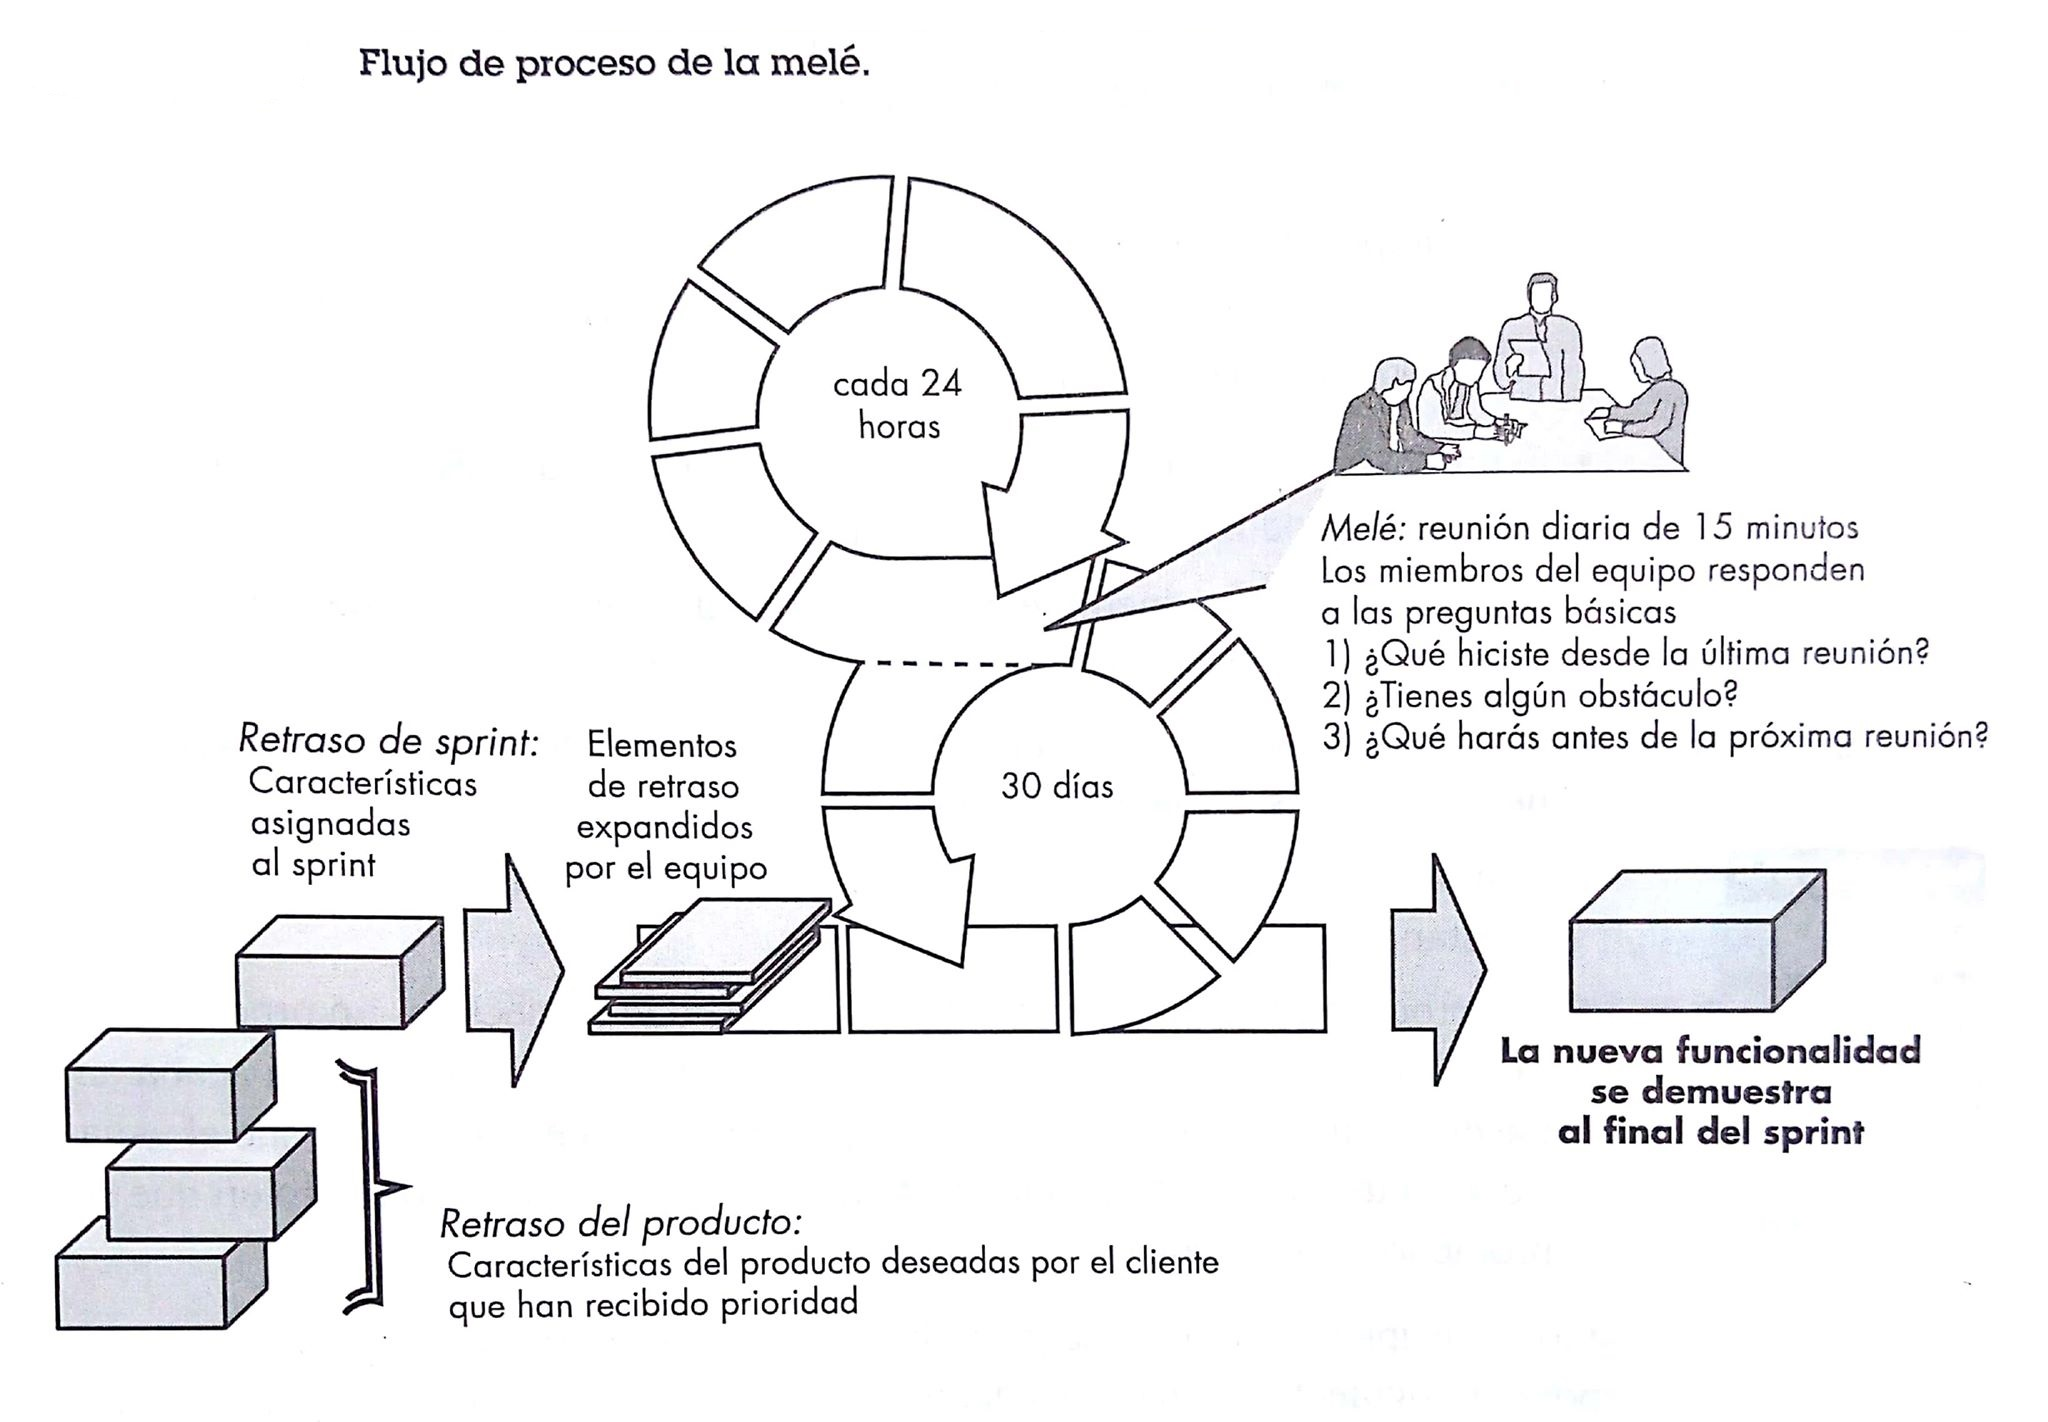
\includegraphics[width=1.2\textwidth]{Imagenes/mele.jpg}
%  \caption{Mi Figura}
%  \label{fig:ejemplo}
%\end{figure}

